\subsection{Punto de Vista del Negocio}
El punto de vista del negocio muestra servicios, eventos y procesos de negocio. Estos son ofrecidos a los diferentes clientes externos que pueden existir. Los servicios son ejecutados por los procesos de negocio, que son el centro de la organización y a su vez son realizados por los diferentes roles.

\subsubsection{Punto de vista de organización}
Se busca encontrar el recurso humano sobre el cual va a recaer nuestro trabajo, y hacer una distribución jerárquica de esa estructura. Se centra en la organización interna de cualquier entidad organizativa,
la cual puede ser una compañía, departamento o entidad organizacional.
Este punto de vista es útil al momento de identificar competencias,
autoridad y responsabilidades.

En el siguiente meta-modelo se muestra como se relacionan los actores,
roles e interfaces permitiendo conocer la responsabilidad y jerarquía
dentro de la organización

\subsubsection{Punto de Vista de Función de Negocio}
El punto de vista de función de negocio muestra la principal función de negocio de una organización y sus relaciones en términos de flujos de información, valor o bienes entre ellos.
Las funciones de la empresa se utilizan para representar los aspectos más estables de una empresa en términos de las actividades primarias que realiza, independientemente de los cambios de organización o desarrollos tecnológicos.

Por lo tanto, la arquitectura función de negocio de las empresas que operan en el mismo mercado a menudo presentan grandes similitudes. Así pues, el punto de vista de la función empresarial proporciona una visión de alto nivel en las operaciones generales de la empresa, y se puede utilizar para identificar las competencias necesarias, o para estructurar una organización  de acuerdo a sus actividades principales

Este punto de vista pretende mostrar las principales funciones de negocio de la organización, denotando las relaciones más importantes entre estas. En el siguiente meta-modelo se muestra el comportamiento interno realizado específicamente por un rol de negocio.

\begin{figure}[th!]
	\centering
	\fcolorbox{black}{white}{
		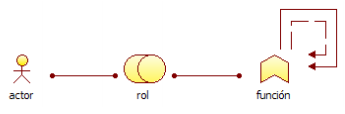
\includegraphics[width=0.7\linewidth]{imgs/puntos_vista/negocio/vistaFuncionNegocio.png}}
	\caption{Modelo de Organización}
	\label{fig:morganizacion}
\end{figure}

\subsubsection{Punto de Vista de Proceso de Negocio}
Otorga claridad de como trabaja la organización, sus insumos y sus resultados.
En un proceso puede fluir información y éste puede disparar información hacia otros procesos o incluso disparar eventos de negocio y otros procesos. Los procesos son asignados a roles y estas son asignadas a roles, el servicio de aplicación es el vinculo entre la capa de negocio y capa de software. Entre sus principales características encontramos:

\begin{itemize}
	\item La asignación de los procesos de negocio a los roles quienes dan la visión de las responsabilidades de los actores asociados.
	\item La información utilizada por los procesos de negocio.
\end{itemize}
\begin{figure}[th!]
	\centering
	\fcolorbox{black}{white}{
		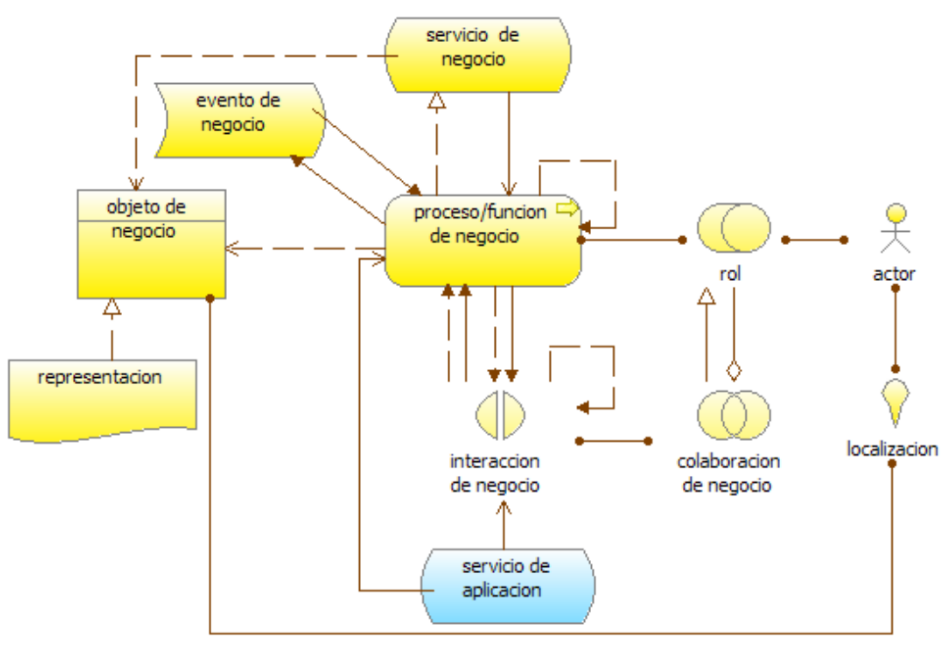
\includegraphics[width=0.9\linewidth]{imgs/puntos_vista/negocio/vistaProcesoNegocio.PNG}}
	\caption{Modelo de Organización}
	\label{fig:morganizacion}
\end{figure}

\subsubsection{Punto de Vista de Cooperación de Proceso de Negocio}
A través de este es posible mostrar la relación entre uno o más procesos de negocio con cada uno y/o con su entorno. Provee las dependencias entre procesos de negocio.

Entre las principales características del punto de vista de cooperación de negocio encontramos:
\begin{itemize}
	\item Relaciones entre los procesos de negocio macro de la compañía.
	\item Mapeo de los procesos de negocio con las funciones de negocio.
	\item Relación entre servicio y procesos de negocio.
	\item Uso de datos compartidos
\end{itemize}

\begin{figure}[th!]
	\centering
	\fcolorbox{black}{white}{
		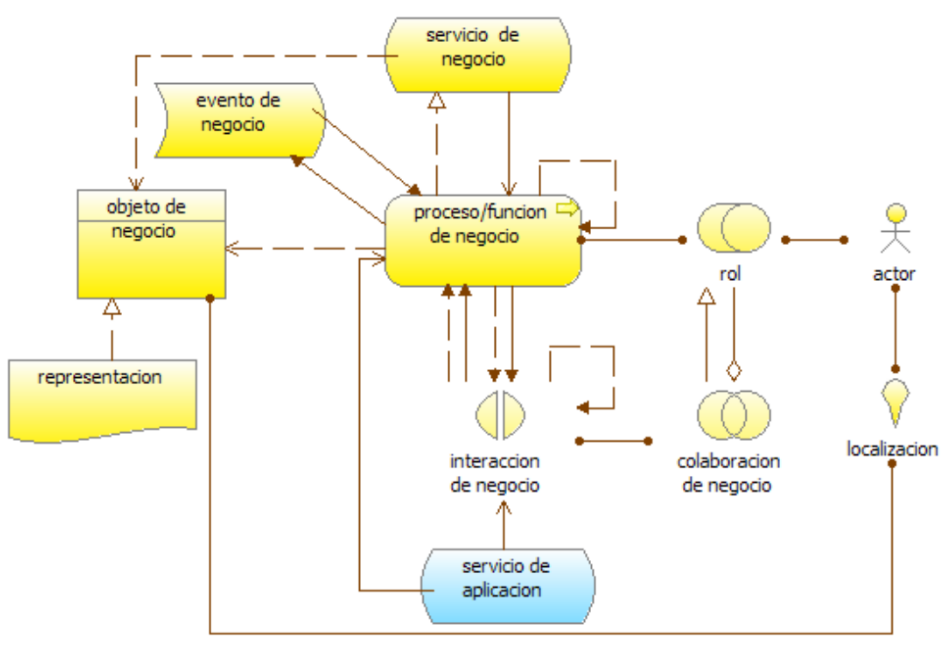
\includegraphics[width=0.9\linewidth]{imgs/puntos_vista/negocio/vistaProcesoNegocio.PNG}}
	
	\label{fig:morganizacion}
\end{figure}

\subsubsection{Punto de Vista de Producto}
Permite el diseño de un producto mediante la composición de servicios existentes o identificando cuales nuevos servicios se pueden crear, con este punto de vista es posible visualizar el output de esta capa. (Lo más importante, el producto) Se materializa el output organizacional del cual se vive.

El producto es conjunto de servicios que se debe buscar justificar, el producto configura un conjunto de contratos.
Lo visible para el cliente es la realización concebida a través de los procesos y los sub-procesos. Se construye a través de un proceso y sus subprocesos.